In table \ref{effects1} and table \ref{effects2}, you can see the main effects and the interaction effects. As one can see, the effect of $B$ is a lot larger than the other effects. This is also shown in the Pareto plot, figure \ref{fig:pareto}. If we should judge from the Pareto plot, $B$ would be the only significant effect.

\begin{table}[H] \centering 
  \caption{Effects} 
  \label{effects1} 
\begin{tabular}{@{\extracolsep{5pt}} cccccccc} 
\\[-1.8ex]\hline 
\hline \\[-1.8ex] 
(Intercept) & A1 & B1 & C1 & D1 & A1:B1 & A1:C1 & A1:D1\\ 
$282.125$ & $$-$1.125$ & $$-$99.875$ & $12.875$ & $4.375$ & $$-$3.125$ & $2.625$ & $$-$3.875$\\ 
\hline \\[-1.8ex] 
\end{tabular} 
\end{table}

\begin{table}[H] \centering 
  \caption{Effects} 
  \label{effects2} 
\begin{tabular}{@{\extracolsep{5pt}} cccccccc} 
\\[-1.8ex]\hline 
B1:C1 & B1:D1 & C1:D1 & A1:B1:C1 & A1:B1:D1 & A1:C1:D1 & B1:C1:D1 & A1:B1:C1:D1\\ 
-13.125 & -6.625 & 2.125 & -10.375 & 1.125 & -13.125 & -15.875 & 7.875\\ 
\hline \\[-1.8ex] 
\end{tabular} 
\end{table}


\begin{figure}[H]
    \centering
    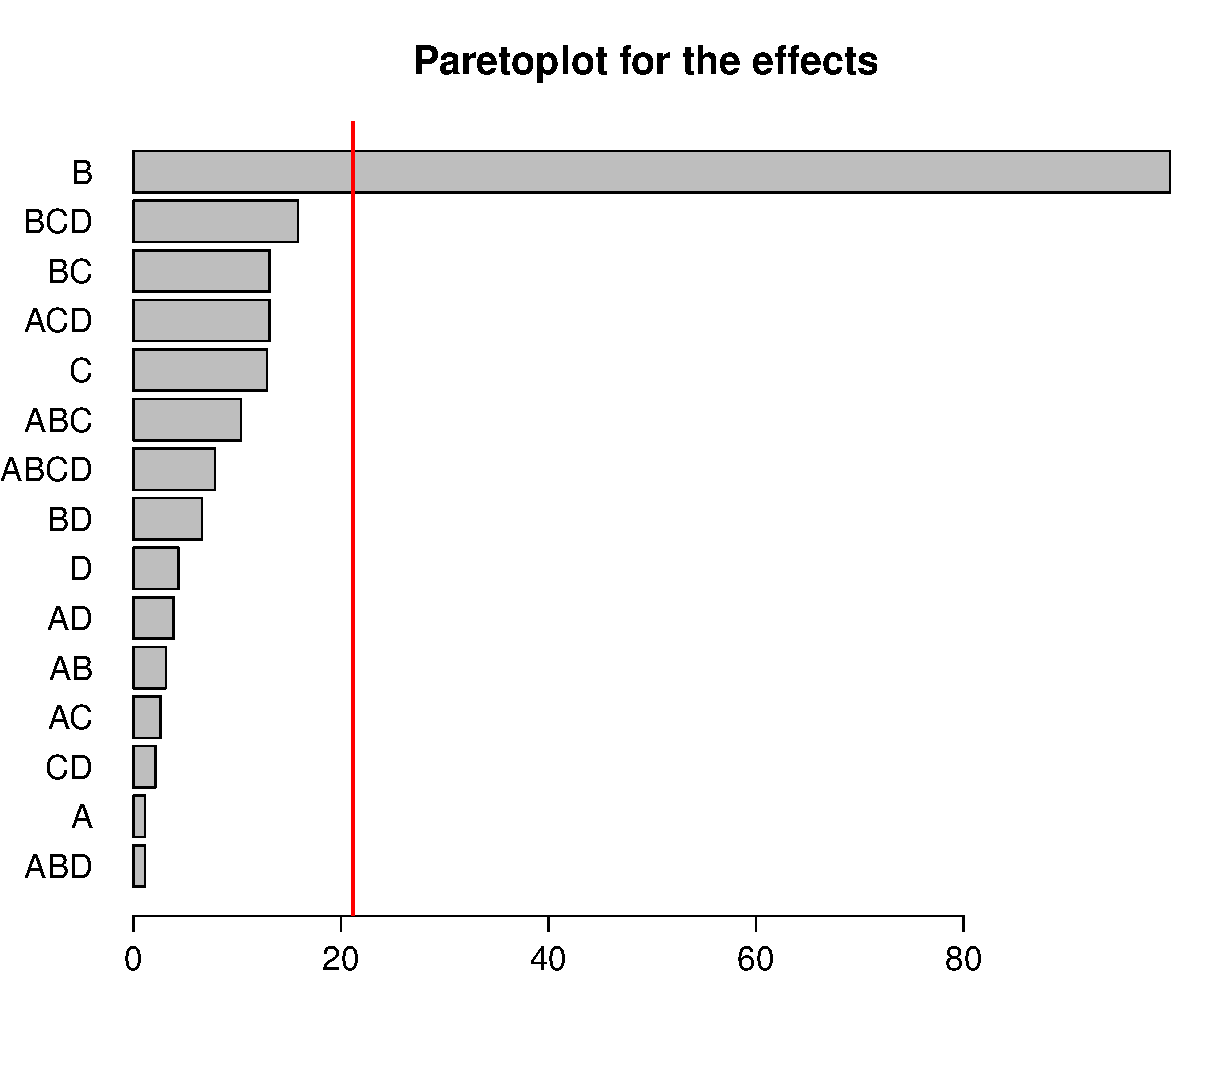
\includegraphics[width=0.6\textwidth]{PDF/paretoPlot.pdf}
    \caption{Pareto plot}
    \label{fig:pareto}
\end{figure}
%
From the main effects plot, figure \ref{fig:mainEff}, it is easy to see that the heating time for the low level is a lot longer than the heating time for the high level. The other three factors show a very small change when going from low to high level.

\begin{figure}[H]
    \centering
    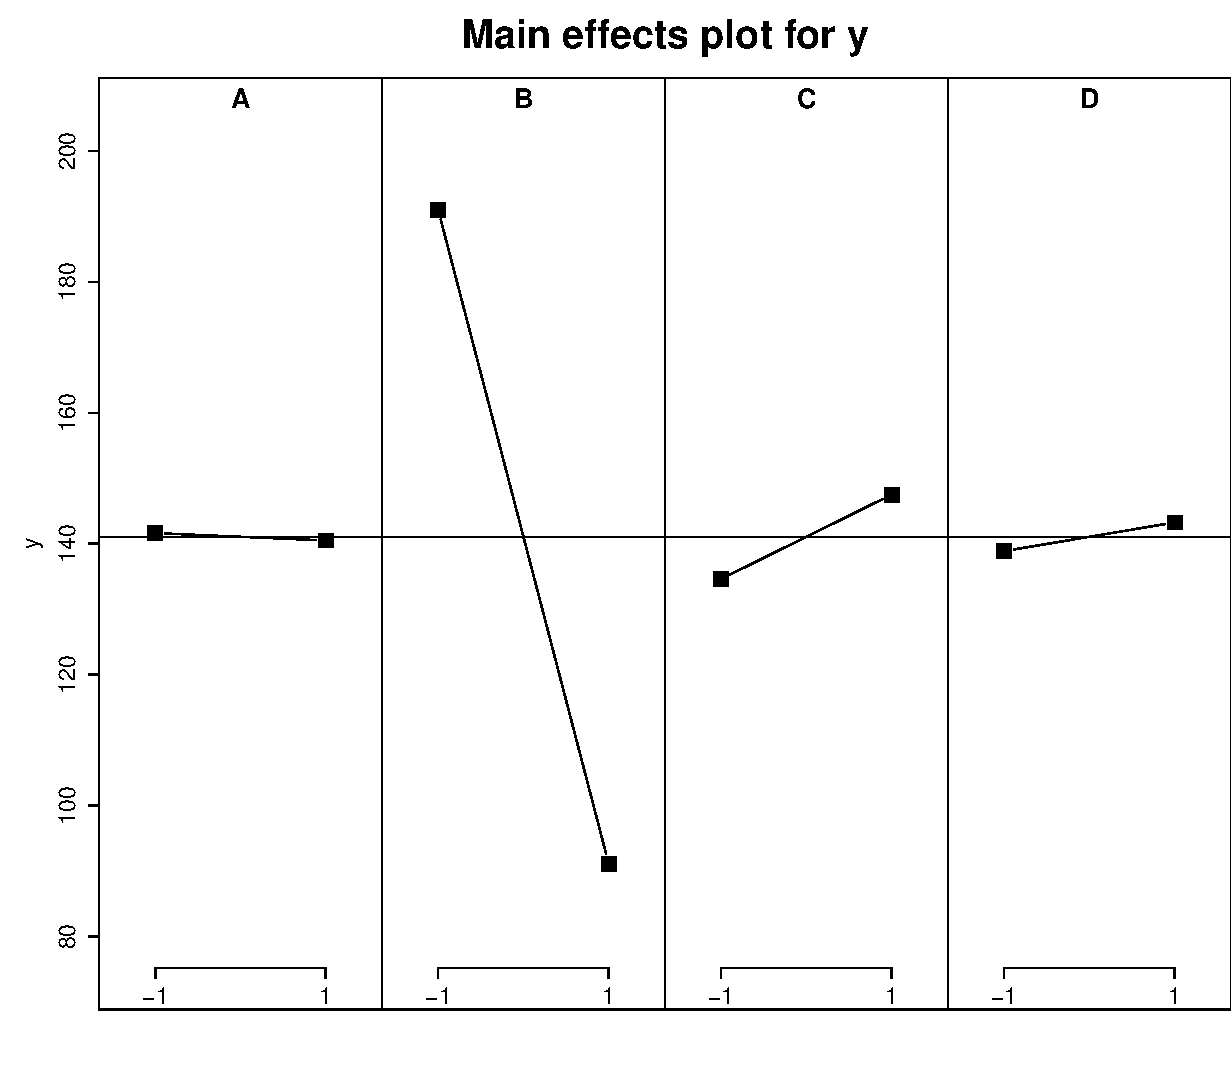
\includegraphics[width=0.6\textwidth]{PDF/mainEffects4factors.pdf}
    \caption{Main effects for y}
    \label{fig:mainEff}
\end{figure}

The interaction effect plot, figure \ref{fig:interaction} does not bring forth any new information. The lines are mostly parallel, except  for the interaction between $B$ and $C$.

\begin{figure}[H]
    \centering
    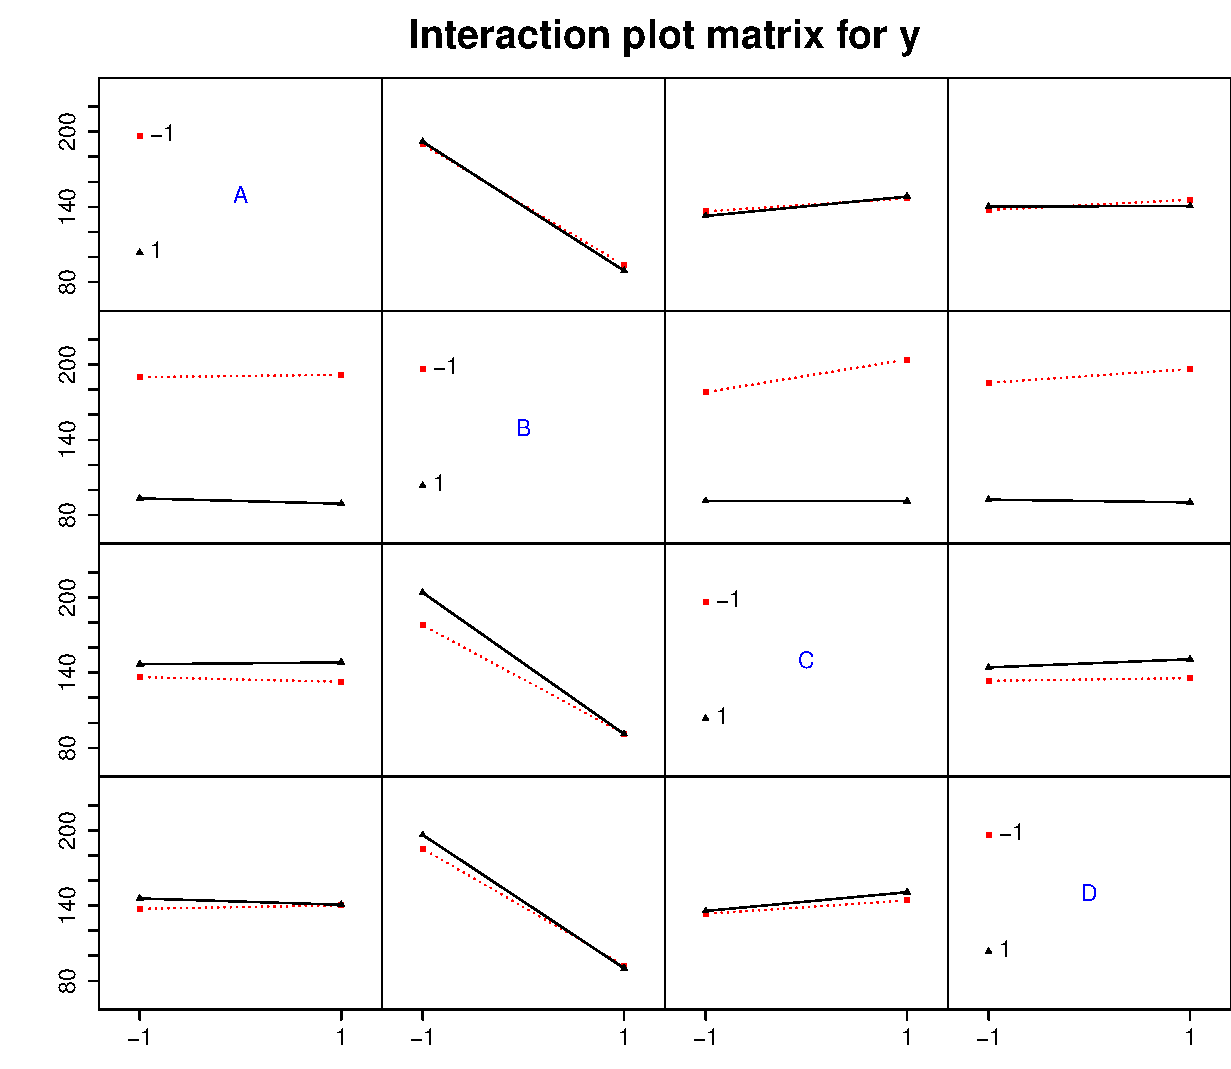
\includegraphics[width=0.6\textwidth]{PDF/interactionPlot4factors.pdf}
    \caption{Interaction effects}
    \label{fig:interaction}
\end{figure}

On the analysis of influence, we used the Cook's Distance as an estimate. In our search for outliers, this test is a good indication of points that merit closer examination in our analysis. Table \ref{Cook} shows the cooks distance for the model where third and fourth-order interaction effects are assumed to be zero. An operational guideline for the D-value is that measurements where $D>1$ should be looked upon more closely. It is seen by \ref{Cook} that this is not the case for our model.

\begin{table}[!htbp] \centering 
  \caption{The Cook's distance}
  \label{Cook} 
\begin{tabular}{@{\extracolsep{5pt}} cccccccc} 
\\[-1.8ex]\hline 
\hline \\[-1.8ex] 
1 & 2 & 3 & 4 & 5 & 6 & 7 & 8 \\ 
0.715 & 0.069 & 0.133 & 0.047 & 0.786 & 0.093 & 0.164 & 0.031\\  \hline
9 & 10 & 11 & 12 & 13 & 14 & 15 & 16 \\
0.216 & 0.014 & 0.0003 & 0.358 & 0.256 & 0.006 & 0.001 & 0.310 \\
\hline \\[-1.8ex] 
\end{tabular} 
\end{table} 

By looking at the residual plot, figure \ref{fig:residual}, a strange pattern emerges. Although it looks like the points are spread out on the y-axis, they are centered in two areas at the x-axis.

\begin{figure}[H]
    \centering
    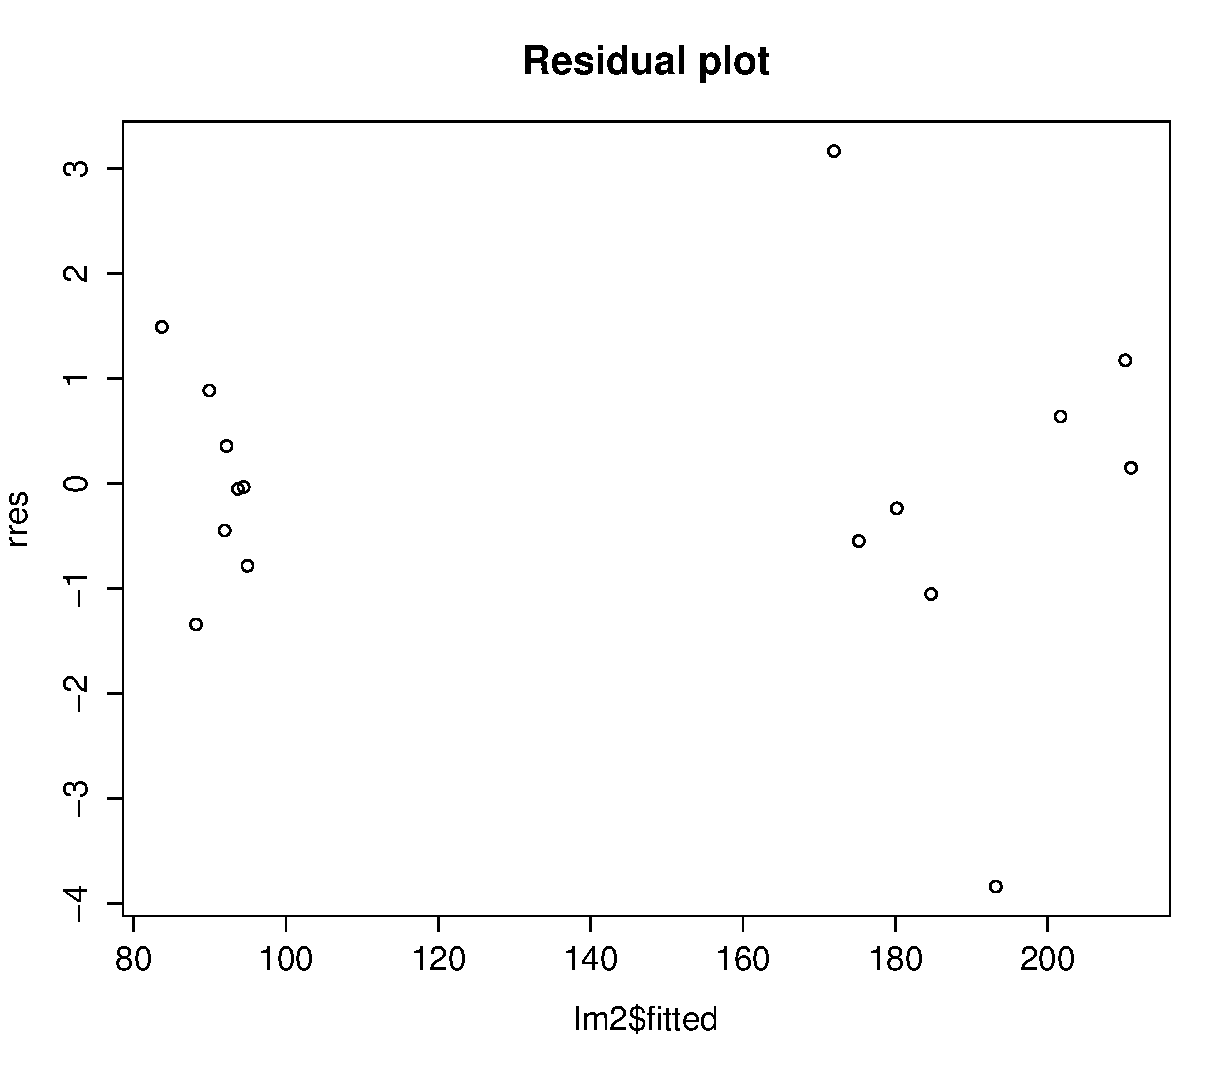
\includegraphics[width=0.6\textwidth]{PDF/residualPlot.pdf}
    \caption{Residual plot}
    \label{fig:residual}
\end{figure}

The Anderson-Darling test is a well know test for normality. For our model with third- and fourth-order interactions removed, the test resulted in a p-value of $0.2646$. Since $p > 0.05$, this p-value supports normality of the data.

On the analysis of influence, we used the Cook's Distance as an estimate. In our search for outliers, this test is a good indication of points that merit closer examination in our analysis.

To further investigate the distribution of the errors, a QQ-plot was made, figure \ref{fig:qqPlot}. This shows that it is normally distributed. All the measurements follow the line, except for two points.

\begin{figure}[H]
    \centering
    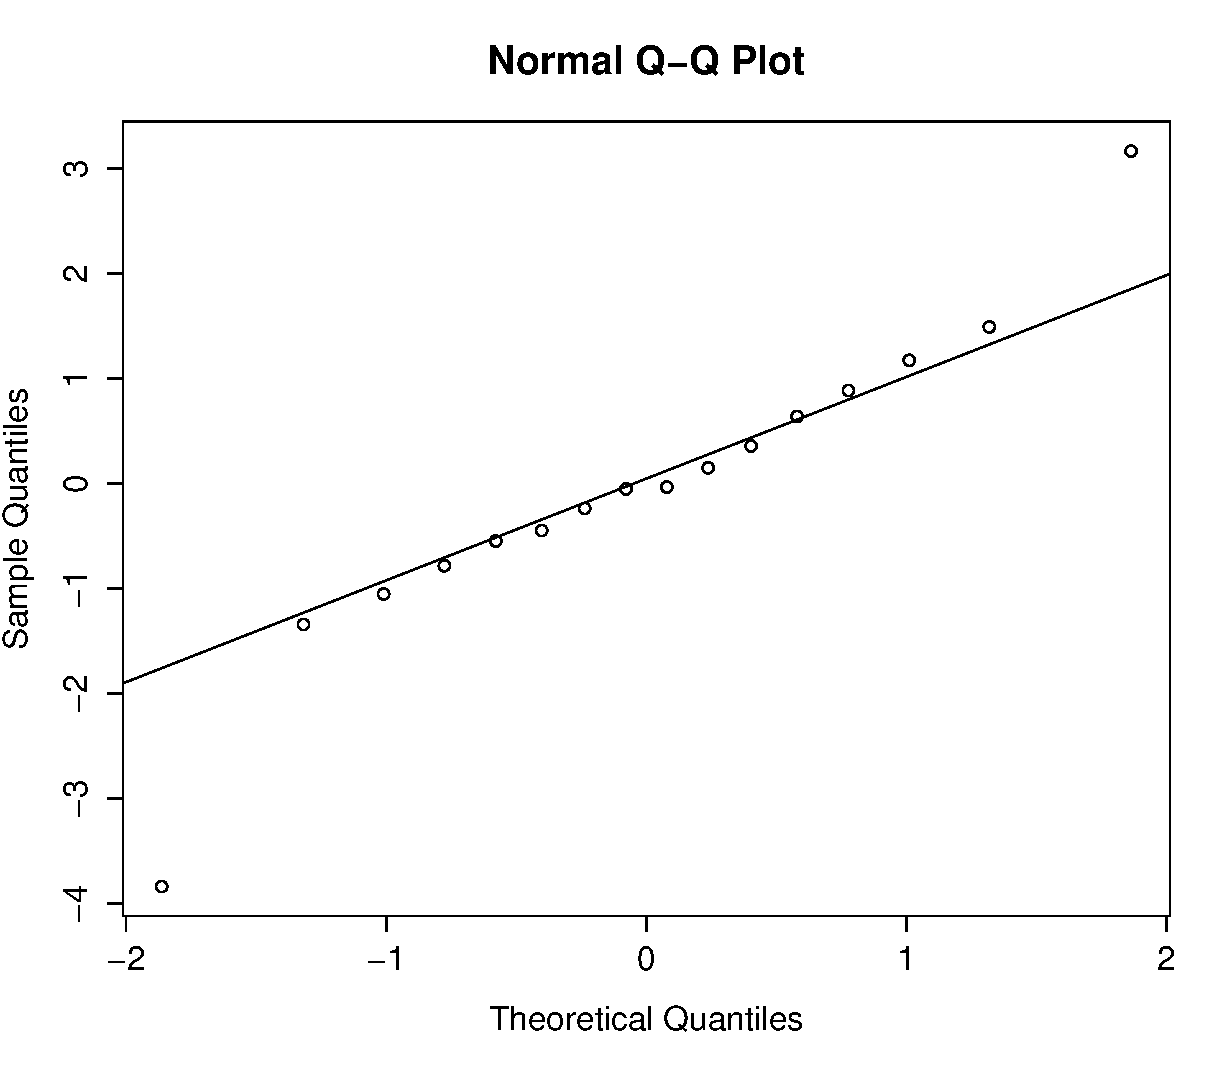
\includegraphics[width=0.6\textwidth]{PDF/qqPlot.pdf}
    \caption{QQ-plot}
    \label{fig:qqPlot}
\end{figure}

Because the residual plot looked a bit strange, the BoxCox-test is performed to see if y needs a transformation. But because $\lambda = 1$ is inside the 95 $\%$ confidence interval, no such transformation is required. 

\begin{figure}[H]
    \centering
    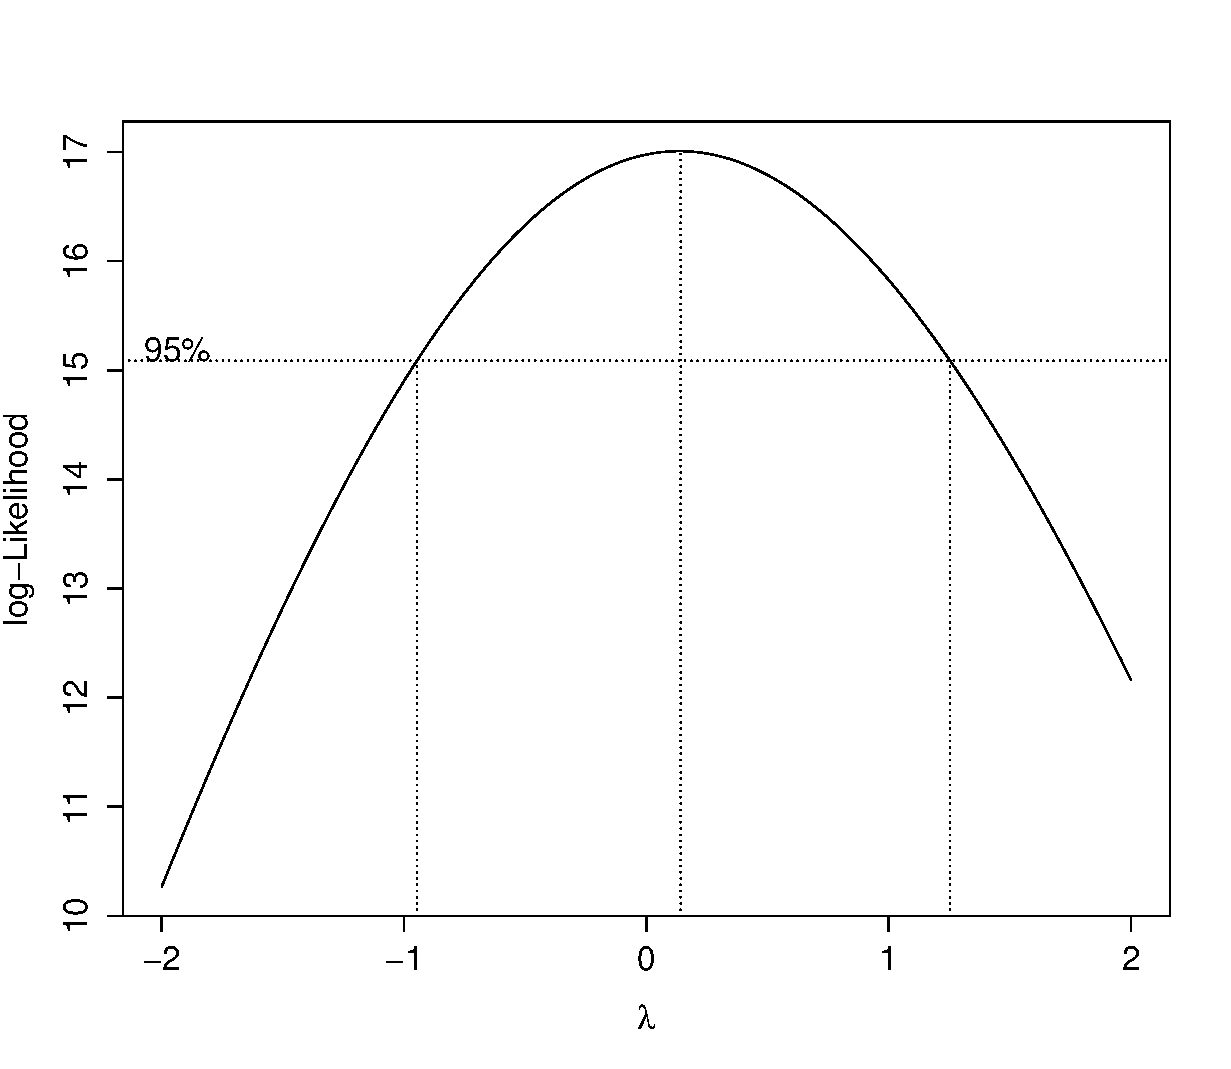
\includegraphics[width=0.6\textwidth]{PDF/boxCox.pdf}
    \caption{BoxCox-plot}
    \label{fig:boxCox}
\end{figure}

\begin{table}[!htbp] \centering 
  \caption{} 
  \label{} 
\begin{tabular}{@{\extracolsep{5pt}} cccccccc} 
\\[-1.8ex]\hline 
\hline \\[-1.8ex] 
1 & 2 & 3 & 4 & 5 & 6 & 7 & 8 \\ 
0.715 & 0.069 & 0.133 & 0.047 & 0.786 & 0.093 & 0.164 & 0.031\\  \hline
9 & 10 & 11 & 12 & 13 & 14 & 15 & 16 \\
0.216 & 0.014 & 0.0003 & 0.358 & 0.256 & 0.006 & 0.001 & 0.310 \\
\hline \\[-1.8ex] 
\end{tabular} 
\end{table}


If the interaction 3-way and 4-way interaction effects are removed, the effects become,
\begin{table}[!htbp] \centering 
  \caption{} 
  \label{} 
\begin{tabular}{@{\extracolsep{5pt}} ccccccccccc} 
\\[-1.8ex]\hline 
\hline \\[-1.8ex] 
(Intercept) & A1 & B1 & C1 & D1 & A1:B1 \\ 
282.125 & -1.125 & -99.875 & 12.875 & 4.375 & -3.125 \\ \hline
A1:C1 & A1:D1 & B1:C1 & B1:D1 & C1:D1 &\\
2.625 & -3.875 & -13.125 & -6.625 & 2.125 \\ 
\hline \\[-1.8ex] 
\end{tabular} 
\end{table}  